\documentclass{beamer}
\usetheme{CambridgeUS}
%\usecolortheme[RGB={0,0,0}]{structure}
\usepackage{pgfpages}
\usepackage{hyperref}
\usepackage{pdfpc-commands}
\usepackage{epstopdf}
\usepackage{array}
\usepackage{svg}
\usepackage{graphicx}
\usepackage{amsmath}
\usepackage{amsfonts}
\usepackage{amssymb}
\usepackage{bm}
\usepackage{ulem}
\usepackage{xfrac}
\usepackage{dcolumn}
\usepackage{multirow}
\usepackage{caption}
\usepackage{color}
\usepackage{listings}
\usepackage{gensymb}
\usepackage{appendixnumberbeamer}
\usepackage{animate}
%\setbeameroption{show notes}
%\setbeameroption{show notes on second screen=right}
\setbeamertemplate{bibliography item}[text]
%\renewcommand{\arraystretch}{1.5}
\newcommand{\mytilde}{\raise.17ex\hbox{$\scriptstyle\mathtt{\sim}$}}
\title[4D Breast Phantom]{Towards a 4D Breast Phantom for Radiotherapy QA}
\author[C. Lund, V.J. Heng]{Chris Lund and Veng Jean Heng}
\titlegraphic{\includegraphics[width=0.5\linewidth]{/home/chris/Documents/McGill/MDPH607/Project/MUHC.jpg}}
\institute[McGill MPU]{Medical Physics Unit \\ Department of Oncology, McGill University}
\date{\today}
%\logo{\includegraphics[scale=0.2]{/home/chris/Documents/McGill/MDPH603/McGill_logo.png}}

\begin{document}

\begin{frame}

    \maketitle

\end{frame}

\begin{frame}

    \frametitle{Motivation}

    \begin{columns}
        \begin{column}{0.5\textwidth}
            \begin{itemize}
                \item Motion in imaging and treatment can pose an issue..
                    \begin{itemize}
                        \item Breath hold/gated treatments
                        \item CyberKnife motion-tracking
                        \item Motion artifacts in IGRT
                    \end{itemize}
                \vspace{1em}
                \item Currently, only available QA phantom is by QUASAR
                    \begin{itemize}
                        \item Very expensive
                        \item Not full 4D capabilities
                    \end{itemize}
                    \vspace{1em}
                \item Desire for open-source alternative
            \end{itemize}
        \end{column}
        \begin{column}{0.5\textwidth}
            \vspace*{-1.5em}
            \begin{figure}[h]
                \centering
                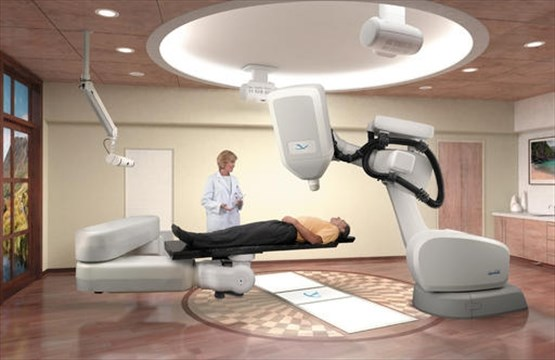
\includegraphics[width=0.9\columnwidth]{cyberknife.jpeg}
            \end{figure}
            \vspace*{-2em}
            \begin{figure}[h]
                \centering
                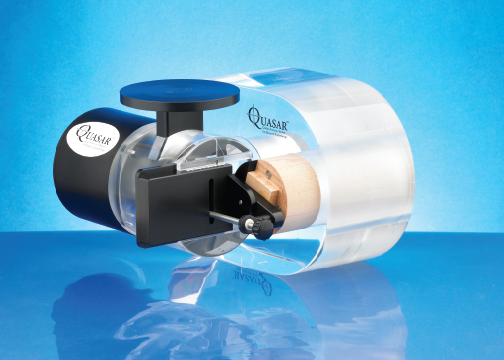
\includegraphics[width=0.9\columnwidth]{QASAR.png}
            \end{figure}
        \end{column}
    \end{columns}

\end{frame}

\begin{frame}

    \frametitle{Overview of Project}

    \begin{itemize}
        \item Want to
            \begin{itemize}
                \item Take in a breathing trace
                \item Convert it into mechanical motion
            \end{itemize}
            \vspace{1em}
        \item Needs to be
            \begin{itemize}
                \item Standalone
                \item ``Perfect'' temporal and spatial accuracy
                \item Open-source and cheap
            \end{itemize}
            \vspace{1em}
        \item How to?
            \begin{itemize}
                \item Raspberry Pi $\rightarrow$ Stepper motor
                \item Rotational motion $\rightarrow$ Linear motion
            \end{itemize}
    \end{itemize}

\end{frame}

\begin{frame}

    \frametitle{Circuitry}

        \begin{figure}
            \centering
            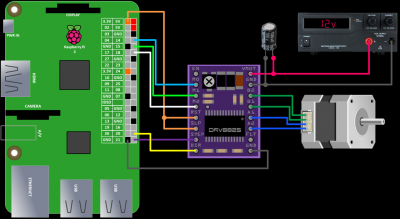
\includegraphics[width=\textwidth]{connections.png}
        \end{figure}

\end{frame}

\begin{frame}

    \frametitle{Stepper Motors}
    \begin{columns}
        \begin{column}{0.5\textwidth}

            \begin{itemize}
                \item Step-based
                    \begin{itemize}
                        \item Define the angle of rotation
                        \item Perfect spatial accuracy
                    \end{itemize}
                    \vspace{1em}
                \item PWM-based
                    \begin{itemize}
                        \item Define the frequency of rotation
                        \item Perfect temporal accuracy
                    \end{itemize}
            \end{itemize}
        \end{column}
        \begin{column}{0.5\textwidth}
            \begin{figure}
                \centering
                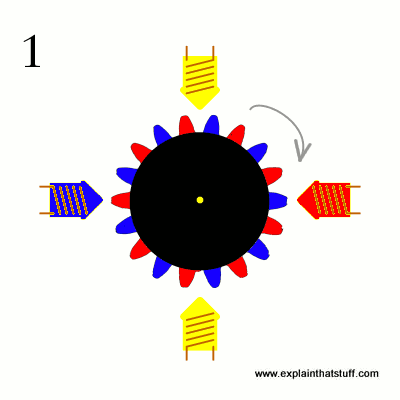
\includegraphics[width=\columnwidth]{steppermotorimage-0.png}
            \end{figure}
        \end{column}
    \end{columns}

                
\end{frame}

\begin{frame}

    \frametitle{Visit our page!}

    \centering
    \url{https://github.com/clund12/MDPH612-project}

\end{frame}


\end{document}
